% BART model as a graphical model with its equations, in the style of
% Lee & Wagenmakers (2013), Bayesian Cognitive Modeling:
%   circle = continuous, square = discrete,
%   shaded = observed / known, unshaded = latent,
%   double border = deterministic, plates = replications.
% Amber outline = quantities the expert is asked about in the app.
%
% Rendered to ../../case_studies/bart_model.png by:  ./render_model.sh
\documentclass[border=8pt]{standalone}
\usepackage{amsmath}
\usepackage{tikz}
\usetikzlibrary{positioning,fit,arrows.meta,calc}

\definecolor{ink}{HTML}{1F2A44}
\definecolor{paper}{HTML}{FFFDF8}
\definecolor{shade}{HTML}{D9D6CF}
\definecolor{elicit}{HTML}{C98A1B}

\tikzset{
  every picture/.style={ink, line width=0.7pt},
  var/.style={draw, minimum size=11mm, inner sep=1pt, text=ink},
  latent/.style={var, circle},
  known/.style={var, circle, fill=shade},
  det/.style={var, circle, double, double distance=1.4pt},
  obsdisc/.style={var, rectangle, fill=shade},
  detdisc/.style={var, rectangle, double, double distance=1.4pt},
  elicited/.style={draw=elicit, line width=1.6pt},
  edge/.style={-{Latex[length=2.4mm]}, line width=0.8pt},
  plate/.style={draw, rounded corners=2pt, inner sep=9pt, line width=0.7pt},
  platelabel/.style={font=\small, anchor=south east, inner sep=3pt},
}

\begin{document}
\pagecolor{paper}% same as the app's panels, so the image has no visible edge
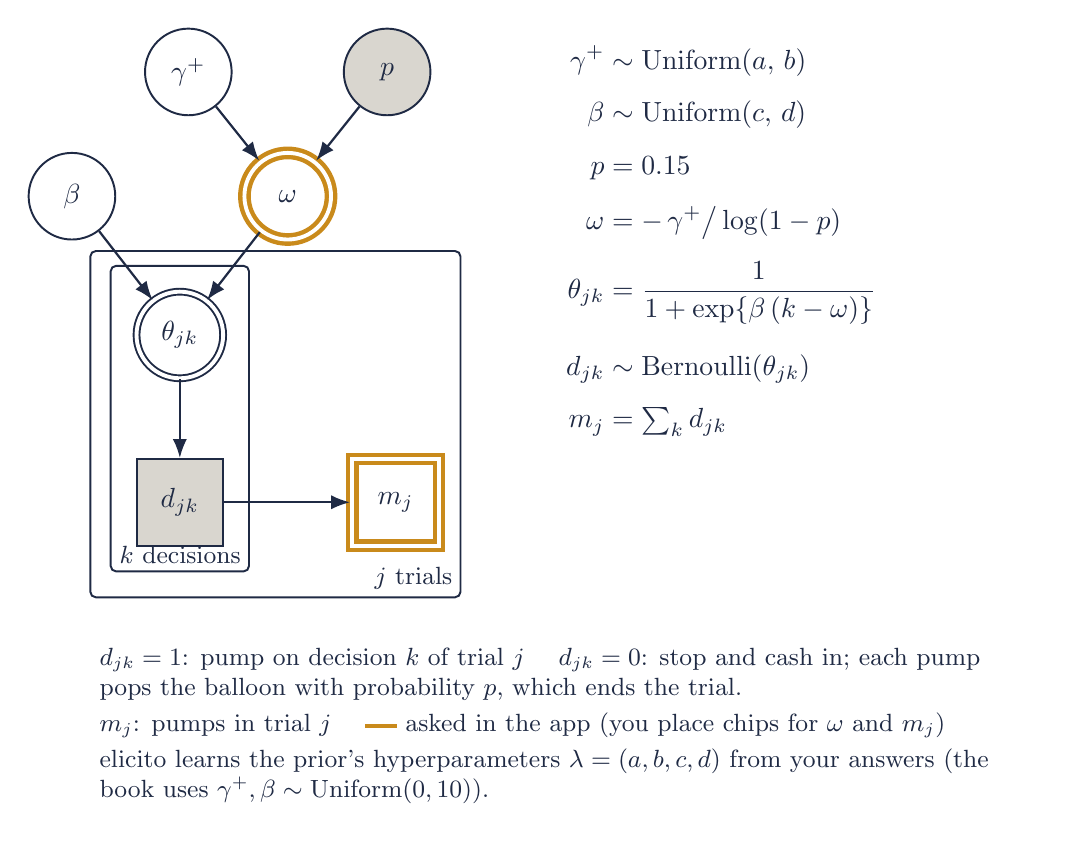
\begin{tikzpicture}
  % ---- graphical model ------------------------------------------------
  \node[latent]                       (gamma) {$\gamma^{+}$};
  \node[known,  right=14mm of gamma]  (p)     {$p$};
  \node[det, elicited, below=10mm of $(gamma)!0.5!(p)$] (omega) {$\omega$};
  \node[latent, left=16mm of omega]   (beta)  {$\beta$};
  \node[det,    below=12mm of $(beta)!0.5!(omega)$] (theta) {$\theta_{jk}$};
  \node[obsdisc, below=10mm of theta] (d)     {$d_{jk}$};
  \node[detdisc, elicited, right=16mm of d] (m) {$m_{j}$};

  \draw[edge] (gamma) -- (omega);
  \draw[edge] (p)     -- (omega);
  \draw[edge] (omega) -- (theta);
  \draw[edge] (beta)  -- (theta);
  \draw[edge] (theta) -- (d);
  \draw[edge] (d)     -- (m);

  \node[plate, fit=(theta)(d)] (inner) {};
  \node[platelabel] at (inner.south east) {$k$ decisions};
  \node[plate, fit=(inner)(m), inner sep=7pt, yshift=-2pt, minimum height=0pt] (outer) {};
  \node[platelabel] at (outer.south east) {$j$ trials};

  % ---- equations ----------------------------------------------------------
  \node[anchor=west, text=ink] at ([xshift=12mm]outer.east |- omega.south) {%
    $\begin{aligned}
      \gamma^{+} &\sim \operatorname{Uniform}(a,\, b) \\[4pt]
      \beta      &\sim \operatorname{Uniform}(c,\, d) \\[4pt]
      p          &= 0.15 \\[4pt]
      \omega     &= -\,\gamma^{+} \big/ \log(1-p) \\[4pt]
      \theta_{jk} &= \dfrac{1}{1 + \exp\{\beta\,(k-\omega)\}} \\[6pt]
      d_{jk}     &\sim \operatorname{Bernoulli}(\theta_{jk}) \\[4pt]
      m_{j}      &= \textstyle\sum_{k} d_{jk}
    \end{aligned}$%
  };

  % ---- notes ------------------------------------------------------------------
  \node[anchor=north west, text=ink, font=\small, align=flush left, text width=118mm]
    at ([yshift=-5mm]outer.south west) {%
    $d_{jk}=1$: pump on decision $k$ of trial $j$ \quad $d_{jk}=0$: stop and cash in;
    each pump pops the balloon with probability $p$, which ends the trial.\\[2pt]
    $m_j$: pumps in trial $j$ \quad
    \textcolor{elicit}{\rule[0.3ex]{4mm}{1.6pt}}\ asked in the app (you place chips for $\omega$ and $m_j$)\\[2pt]
    elicito learns the prior's hyperparameters $\lambda = (a, b, c, d)$ from your answers
    (the book uses $\gamma^{+}, \beta \sim \operatorname{Uniform}(0, 10)$).
  };
\end{tikzpicture}
\end{document}
